\PassOptionsToPackage{unicode=true}{hyperref} % options for packages loaded elsewhere
\PassOptionsToPackage{hyphens}{url}
%
\documentclass[]{article}
\usepackage{lmodern}
\usepackage{amssymb,amsmath}
\usepackage{ifxetex,ifluatex}
\usepackage{fixltx2e} % provides \textsubscript
\ifnum 0\ifxetex 1\fi\ifluatex 1\fi=0 % if pdftex
  \usepackage[T1]{fontenc}
  \usepackage[utf8]{inputenc}
  \usepackage{textcomp} % provides euro and other symbols
\else % if luatex or xelatex
  \usepackage{unicode-math}
  \defaultfontfeatures{Ligatures=TeX,Scale=MatchLowercase}
\fi
% use upquote if available, for straight quotes in verbatim environments
\IfFileExists{upquote.sty}{\usepackage{upquote}}{}
% use microtype if available
\IfFileExists{microtype.sty}{%
\usepackage[]{microtype}
\UseMicrotypeSet[protrusion]{basicmath} % disable protrusion for tt fonts
}{}
\IfFileExists{parskip.sty}{%
\usepackage{parskip}
}{% else
\setlength{\parindent}{0pt}
\setlength{\parskip}{6pt plus 2pt minus 1pt}
}
\usepackage{hyperref}
\hypersetup{
            pdftitle={Project 2 (Modeling)},
            pdfauthor={Jaqueline Ma},
            pdfborder={0 0 0},
            breaklinks=true}
\urlstyle{same}  % don't use monospace font for urls
\usepackage[margin=1in]{geometry}
\usepackage{color}
\usepackage{fancyvrb}
\newcommand{\VerbBar}{|}
\newcommand{\VERB}{\Verb[commandchars=\\\{\}]}
\DefineVerbatimEnvironment{Highlighting}{Verbatim}{commandchars=\\\{\}}
% Add ',fontsize=\small' for more characters per line
\usepackage{framed}
\definecolor{shadecolor}{RGB}{248,248,248}
\newenvironment{Shaded}{\begin{snugshade}}{\end{snugshade}}
\newcommand{\AlertTok}[1]{\textcolor[rgb]{0.94,0.16,0.16}{#1}}
\newcommand{\AnnotationTok}[1]{\textcolor[rgb]{0.56,0.35,0.01}{\textbf{\textit{#1}}}}
\newcommand{\AttributeTok}[1]{\textcolor[rgb]{0.77,0.63,0.00}{#1}}
\newcommand{\BaseNTok}[1]{\textcolor[rgb]{0.00,0.00,0.81}{#1}}
\newcommand{\BuiltInTok}[1]{#1}
\newcommand{\CharTok}[1]{\textcolor[rgb]{0.31,0.60,0.02}{#1}}
\newcommand{\CommentTok}[1]{\textcolor[rgb]{0.56,0.35,0.01}{\textit{#1}}}
\newcommand{\CommentVarTok}[1]{\textcolor[rgb]{0.56,0.35,0.01}{\textbf{\textit{#1}}}}
\newcommand{\ConstantTok}[1]{\textcolor[rgb]{0.00,0.00,0.00}{#1}}
\newcommand{\ControlFlowTok}[1]{\textcolor[rgb]{0.13,0.29,0.53}{\textbf{#1}}}
\newcommand{\DataTypeTok}[1]{\textcolor[rgb]{0.13,0.29,0.53}{#1}}
\newcommand{\DecValTok}[1]{\textcolor[rgb]{0.00,0.00,0.81}{#1}}
\newcommand{\DocumentationTok}[1]{\textcolor[rgb]{0.56,0.35,0.01}{\textbf{\textit{#1}}}}
\newcommand{\ErrorTok}[1]{\textcolor[rgb]{0.64,0.00,0.00}{\textbf{#1}}}
\newcommand{\ExtensionTok}[1]{#1}
\newcommand{\FloatTok}[1]{\textcolor[rgb]{0.00,0.00,0.81}{#1}}
\newcommand{\FunctionTok}[1]{\textcolor[rgb]{0.00,0.00,0.00}{#1}}
\newcommand{\ImportTok}[1]{#1}
\newcommand{\InformationTok}[1]{\textcolor[rgb]{0.56,0.35,0.01}{\textbf{\textit{#1}}}}
\newcommand{\KeywordTok}[1]{\textcolor[rgb]{0.13,0.29,0.53}{\textbf{#1}}}
\newcommand{\NormalTok}[1]{#1}
\newcommand{\OperatorTok}[1]{\textcolor[rgb]{0.81,0.36,0.00}{\textbf{#1}}}
\newcommand{\OtherTok}[1]{\textcolor[rgb]{0.56,0.35,0.01}{#1}}
\newcommand{\PreprocessorTok}[1]{\textcolor[rgb]{0.56,0.35,0.01}{\textit{#1}}}
\newcommand{\RegionMarkerTok}[1]{#1}
\newcommand{\SpecialCharTok}[1]{\textcolor[rgb]{0.00,0.00,0.00}{#1}}
\newcommand{\SpecialStringTok}[1]{\textcolor[rgb]{0.31,0.60,0.02}{#1}}
\newcommand{\StringTok}[1]{\textcolor[rgb]{0.31,0.60,0.02}{#1}}
\newcommand{\VariableTok}[1]{\textcolor[rgb]{0.00,0.00,0.00}{#1}}
\newcommand{\VerbatimStringTok}[1]{\textcolor[rgb]{0.31,0.60,0.02}{#1}}
\newcommand{\WarningTok}[1]{\textcolor[rgb]{0.56,0.35,0.01}{\textbf{\textit{#1}}}}
\usepackage{graphicx,grffile}
\makeatletter
\def\maxwidth{\ifdim\Gin@nat@width>\linewidth\linewidth\else\Gin@nat@width\fi}
\def\maxheight{\ifdim\Gin@nat@height>\textheight\textheight\else\Gin@nat@height\fi}
\makeatother
% Scale images if necessary, so that they will not overflow the page
% margins by default, and it is still possible to overwrite the defaults
% using explicit options in \includegraphics[width, height, ...]{}
\setkeys{Gin}{width=\maxwidth,height=\maxheight,keepaspectratio}
\setlength{\emergencystretch}{3em}  % prevent overfull lines
\providecommand{\tightlist}{%
  \setlength{\itemsep}{0pt}\setlength{\parskip}{0pt}}
\setcounter{secnumdepth}{0}
% Redefines (sub)paragraphs to behave more like sections
\ifx\paragraph\undefined\else
\let\oldparagraph\paragraph
\renewcommand{\paragraph}[1]{\oldparagraph{#1}\mbox{}}
\fi
\ifx\subparagraph\undefined\else
\let\oldsubparagraph\subparagraph
\renewcommand{\subparagraph}[1]{\oldsubparagraph{#1}\mbox{}}
\fi

% set default figure placement to htbp
\makeatletter
\def\fps@figure{htbp}
\makeatother


\title{Project 2 (Modeling)}
\author{Jaqueline Ma}
\date{}

\begin{document}
\maketitle

\hypertarget{introduction}{%
\section{Introduction}\label{introduction}}

For this project, I chose the `studentdata' dataset from the LearnBayes
package in Rstudio. In this dataset, the variables consisted of Student
(which is the student number), Height, Gender, Shoes (the number of
pairs of shoes owned), Number (number chosen between 1 and 10), Dvds
(number of movie dvds owned), ToSleep (time the person went to sleep the
previous night -hours past midnight), WakeUp (time the person woke up
the next morning), Haircut (cost of last haircut including tip), Job
(number of hours working on a job per week), and Drink (usual drink at
suppertime among milk, water and pop). There are 657 observations and
the variable of gender was dummy coded under a new variable called
\(y\). The NAs and the Student variable were also omitted to allow for
easier data analysis, leading to a total of 559 observations.

\begin{Shaded}
\begin{Highlighting}[]
\KeywordTok{library}\NormalTok{(LearnBayes)}
\KeywordTok{head}\NormalTok{(studentdata)}
\end{Highlighting}
\end{Shaded}

\begin{verbatim}
## Student Height Gender Shoes Number Dvds ToSleep WakeUp
Haircut Job Drink
## 1 1 67 female 10 5 10 -2.5 5.5 60 30.0 water
## 2 2 64 female 20 7 5 1.5 8.0 0 20.0 pop
## 3 3 61 female 12 2 6 -1.5 7.5 48 0.0 milk
## 4 4 61 female 3 6 40 2.0 8.5 10 0.0 water
## 5 5 70 male 4 5 6 0.0 9.0 15 17.5 pop
## 6 6 63 female NA 3 5 1.0 8.5 25 0.0 water
\end{verbatim}

\begin{Shaded}
\begin{Highlighting}[]
\NormalTok{students <-}\StringTok{ }\NormalTok{studentdata}\OperatorTok\KeywordTok{mutate}\NormalTok{(}\DataTypeTok{y =} \KeywordTok{ifelse}\NormalTok{(Gender }\OperatorTok{==}\StringTok{ "male"}\NormalTok{, }\DecValTok{1}\NormalTok{, }\DecValTok{0}\NormalTok{))}\OperatorTok\NormalTok{na.omit}
\NormalTok{students}\OperatorTok{$}\NormalTok{Student <-}\StringTok{ }\OtherTok{NULL}
\NormalTok{students}\OperatorTok\NormalTok{count}
\end{Highlighting}
\end{Shaded}

\begin{verbatim}
## # A tibble: 1 x 1
##       n
##   <int>
## 1   559
\end{verbatim}

\hypertarget{manova-test}{%
\section{MANOVA Test}\label{manova-test}}

For this data, a MANOVA test was conducted to see if any of the response
variables differ by levels of a categorical explanatory variable. The
null hypothesis would be that the means of the response variables are
equal whereas the alternative hypothesis would be that the means of the
response variables are significantly different. I tested the response
variables of Height, and Shoes against the variable of Drink (null = for
the DVs of Height, and Shoes, means for each Drink are equal;
alternative = for at least one DV, at least one Drink mean is
different).

After running the MANOVA, I can reject the null hypothesis and conclude
that there is a mean difference among the three levels of Drink for at
least one of the dependent variables, \emph{Pillai trace} = 0.024356,
\emph{psuedo F} = 3.4273, \emph{p} = 0.008546

Since the overall MANOVA was significant, I performed univariate ANOVAs
for each variable as follow-up tests. The result of these ANOVAs was
that only the univariate ANOVA for Shoes was significant; for Shoes, at
least one Drink differs (the other variable was not significant),
\emph{F} = 5.4281, \emph{p} = 0.004627.

Post hoc analysis was performed conducting pairwise comparisons to
determine which Drink differed by Shoes. Only the Drinks of milk and
water were found to differ significantly from each other after adjusting
for multiple comparisons (bonferroni alpha = 0.05/10 = 0.005)

There were a total of 6 tests performed (1 MANOVA, 2 ANOVAS and 3 post
hoc/t-tests). Based on the number of tests, the probability of at least
1 type I error would be 0.2649081 or 26.5\%. The significance level
would then be adjusted to 0.008333333.

Some assumptions of this test include: random sample, multivariate
normality of dependent variables, homogeneity of within group covariance
matrices and linear relationships among dependent variables. The
multivariate normality was estimated by making multivariate plots of
response variables for each group. Examination of these density plots
revealed a departure from multivariate normality. Random sample might
also be violated since it is not explicit on where this student data
came from. In addition, examination of covariance matrices for each
group revealed differenes and a lack of homogeneity. It is possible that
MANOVA would not be an appropriate analysis technique.

\begin{Shaded}
\begin{Highlighting}[]
\NormalTok{man1 <-}\StringTok{ }\KeywordTok{manova}\NormalTok{(}\KeywordTok{cbind}\NormalTok{(Height, Shoes)}\OperatorTok{~}\NormalTok{Drink, }\DataTypeTok{data =}\NormalTok{ students)}
\KeywordTok{summary}\NormalTok{(man1)}
\end{Highlighting}
\end{Shaded}

\begin{verbatim}
## Df Pillai approx F num Df den Df Pr(>F)
## Drink 2 0.024356 3.4273 4 1112 0.008546 **
## Residuals 556
## ---
## Signif. codes: 0 '***' 0.001 '**' 0.01 '*' 0.05 '.' 0.1
' ' 1
\end{verbatim}

\begin{Shaded}
\begin{Highlighting}[]
\KeywordTok{summary.aov}\NormalTok{(man1)}
\end{Highlighting}
\end{Shaded}

\begin{verbatim}
## Response Height :
## Df Sum Sq Mean Sq F value Pr(>F)
## Drink 2 45.7 22.865 1.2943 0.2749
## Residuals 556 9822.0 17.665
##
## Response Shoes :
## Df Sum Sq Mean Sq F value Pr(>F)
## Drink 2 2065 1032.57 5.4281 0.004627 **
## Residuals 556 105767 190.23
## ---
## Signif. codes: 0 '***' 0.001 '**' 0.01 '*' 0.05 '.' 0.1
' ' 1
\end{verbatim}

\begin{Shaded}
\begin{Highlighting}[]
\NormalTok{students}\OperatorTok\KeywordTok{group_by}\NormalTok{(Drink)}\OperatorTok\KeywordTok{summarize}\NormalTok{(}\KeywordTok{mean}\NormalTok{(Height),}\KeywordTok{mean}\NormalTok{(Shoes))}
\end{Highlighting}
\end{Shaded}

\begin{verbatim}
## # A tibble: 3 x 3
##   Drink `mean(Height)` `mean(Shoes)`
##   <fct>          <dbl>         <dbl>
## 1 milk            66.5          12.5
## 2 pop             67.2          14.2
## 3 water           66.6          17.3
\end{verbatim}

\begin{Shaded}
\begin{Highlighting}[]
\KeywordTok{pairwise.t.test}\NormalTok{(students}\OperatorTok{$}\NormalTok{Shoes, students}\OperatorTok{$}\NormalTok{Drink, }\DataTypeTok{p.adj=}\StringTok{"none"}\NormalTok{)}
\end{Highlighting}
\end{Shaded}

\begin{verbatim}
## 
##  Pairwise comparisons using t tests with pooled SD 
## 
## data:  students$Shoes and students$Drink 
## 
##       milk   pop   
## pop   0.3562 -     
## water 0.0034 0.0244
## 
## P value adjustment method: none
\end{verbatim}

\begin{Shaded}
\begin{Highlighting}[]
\CommentTok{#probability}
\DecValTok{1}\FloatTok{-0.95}\OperatorTok{^}\DecValTok{6}
\end{Highlighting}
\end{Shaded}

\begin{verbatim}
## [1] 0.2649081
\end{verbatim}

\begin{Shaded}
\begin{Highlighting}[]
\CommentTok{#bonferroni alpha adjusted}
\FloatTok{0.05}\OperatorTok{/}\DecValTok{6}
\end{Highlighting}
\end{Shaded}

\begin{verbatim}
## [1] 0.008333333
\end{verbatim}

\begin{Shaded}
\begin{Highlighting}[]
\KeywordTok{library}\NormalTok{(mvtnorm)}
\KeywordTok{library}\NormalTok{(ggExtra)}
\KeywordTok{ggplot}\NormalTok{(students, }\KeywordTok{aes}\NormalTok{(}\DataTypeTok{x =}\NormalTok{ Height, }\DataTypeTok{y =}\NormalTok{ Shoes))}\OperatorTok{+}\KeywordTok{geom_point}\NormalTok{(}\DataTypeTok{alpha =} \FloatTok{0.5}\NormalTok{)}\OperatorTok{+}\StringTok{  }
\StringTok{  }\KeywordTok{geom_density_2d}\NormalTok{(}\DataTypeTok{h=}\DecValTok{2}\NormalTok{)}\OperatorTok{+}\KeywordTok{facet_wrap}\NormalTok{(}\OperatorTok{~}\NormalTok{Drink)}
\end{Highlighting}
\end{Shaded}

\begin{center}\includegraphics{project2_files/figure-latex/unnamed-chunk-2-1} \end{center}

\begin{Shaded}
\begin{Highlighting}[]
\NormalTok{covmats<-}\StringTok{ }\NormalTok{students}\OperatorTok\KeywordTok{group_by}\NormalTok{(Drink)}\OperatorTok\KeywordTok{do}\NormalTok{(}\DataTypeTok{covs =} \KeywordTok{cov}\NormalTok{(.[}\KeywordTok{c}\NormalTok{(}\DecValTok{1}\NormalTok{,}\DecValTok{3}\NormalTok{)]))}
\ControlFlowTok{for}\NormalTok{(i }\ControlFlowTok{in} \DecValTok{1}\OperatorTok{:}\DecValTok{3}\NormalTok{)\{}\KeywordTok{print}\NormalTok{(}\KeywordTok{as.character}\NormalTok{(covmats}\OperatorTok{$}\NormalTok{Drink[i]));}\KeywordTok{print}\NormalTok{(covmats}\OperatorTok{$}\NormalTok{covs[i])\}}
\end{Highlighting}
\end{Shaded}

\begin{verbatim}
## [1] "milk"
## [[1]]
##           Height     Shoes
## Height  18.35809 -18.70580
## Shoes  -18.70580  93.78028
## 
## [1] "pop"
## [[1]]
##           Height     Shoes
## Height  17.85651 -15.29649
## Shoes  -15.29649 106.12359
## 
## [1] "water"
## [[1]]
##           Height     Shoes
## Height  17.35355 -24.48873
## Shoes  -24.48873 262.30374
\end{verbatim}

\hypertarget{randomization-test}{%
\section{Randomization Test}\label{randomization-test}}

A randomization test was then performed between the variables of Gender
and Job, to see if there was a difference in the number of hours working
on a job per week between males and females. Assumptions for the
independent t-test were violated. The null hypothesis would be: the mean
number of hours working on a job per week is the same for males and
females while the alternative hypothesis would be: the mean number of
hours working on a job per week is different for males and females.

The actual mean differences between the groups was first found and
calculated to be 0.6631868. Then, the job hours were randomly scrambled
and the mean differences between the gender groups was found from the
randomly scrambled variables; this was done through a vector and for
loop for 5,000 times. A histogram shows the distribution of the
randomized values and the actual mean difference between the original
data (as a red line).

Lastly, the two tailed p-value was calculated to be 0.479, which would
correspond to the probability of observing a mean difference as extreme
as the one I observed in the original data under this randomized
distribution. Therefore, I would fail to reject the null hypothesis and
conclude that there is no significant difference between the mean number
of hours working on a job per week between males and females.

\begin{Shaded}
\begin{Highlighting}[]
\NormalTok{students}\OperatorTok\KeywordTok{group_by}\NormalTok{(Gender)}\OperatorTok\KeywordTok{summarize}\NormalTok{(}\DataTypeTok{means=}\KeywordTok{mean}\NormalTok{(Job))}\OperatorTok\StringTok{  }
\StringTok{  }\KeywordTok{summarize}\NormalTok{(}\StringTok{`}\DataTypeTok{mean_diff:}\StringTok{`}\NormalTok{=}\KeywordTok{diff}\NormalTok{(means))}
\end{Highlighting}
\end{Shaded}

\begin{verbatim}
## # A tibble: 1 x 1
##   `mean_diff:`
##          <dbl>
## 1        0.663
\end{verbatim}

\begin{Shaded}
\begin{Highlighting}[]
\NormalTok{rand_dist<-}\KeywordTok{vector}\NormalTok{()}
\ControlFlowTok{for}\NormalTok{(i }\ControlFlowTok{in} \DecValTok{1}\OperatorTok{:}\DecValTok{5000}\NormalTok{)\{}
\NormalTok{new<-}\KeywordTok{data.frame}\NormalTok{(}\DataTypeTok{gender =}\NormalTok{ students}\OperatorTok{$}\NormalTok{Gender,}\DataTypeTok{job =} \KeywordTok{sample}\NormalTok{(students}\OperatorTok{$}\NormalTok{Job))}
\NormalTok{rand_dist[i]<-}\KeywordTok{mean}\NormalTok{(new[new}\OperatorTok{$}\NormalTok{gender }\OperatorTok{==}\StringTok{ "male"}\NormalTok{,]}\OperatorTok{$}\NormalTok{job)}\OperatorTok{-}\KeywordTok{mean}\NormalTok{(new[new}\OperatorTok{$}\NormalTok{gender }\OperatorTok{==}\StringTok{ "female"}\NormalTok{,]}\OperatorTok{$}\NormalTok{job)\}}

\NormalTok{\{}\KeywordTok{hist}\NormalTok{(rand_dist, }\DataTypeTok{main =} \StringTok{""}\NormalTok{,}\DataTypeTok{ylab =}\StringTok{""}\NormalTok{); }\KeywordTok{abline}\NormalTok{(}\DataTypeTok{v =} \FloatTok{0.6631868}\NormalTok{, }\DataTypeTok{col=}\StringTok{"red"}\NormalTok{)\}}
\end{Highlighting}
\end{Shaded}

\begin{center}\includegraphics{project2_files/figure-latex/unnamed-chunk-3-1} \end{center}

\begin{Shaded}
\begin{Highlighting}[]
\KeywordTok{mean}\NormalTok{(rand_dist}\OperatorTok{>}\FloatTok{0.6631868}\OperatorTok{|}\NormalTok{rand_dist}\OperatorTok{<}\StringTok{ }\FloatTok{-0.6631868}\NormalTok{)}
\end{Highlighting}
\end{Shaded}

\begin{verbatim}
## [1] 0.493
\end{verbatim}

\#Linear Regression Model

Next, a linear regression model was used to predict Height from the
variables of Shoes (number of Shoes) and Gender, while also taking into
consideration their interaction. The variable of Shoes was mean centered
since it was a numeric variable. The null hypotheses would be that
controlling for Shoes, Gender does not explain variation in Height and
that controlling for Gender, Shoes does not explain variation in Height.
In contrast, the alternative hypotheses would be that controlling for
Shoes, Gender does explain variation in Height and that controlling for
Gender, Shoes does explain variation in Height.

Based on these coefficient estimates, when people have the average
number of Shoes, and are female, the average Height will be 64.94709.
When controlling for Shoes, males will have a 5.41655 average increase
in Height compared to females. When the person is a female, there is a
decrease of 0.02413 in Height for every 1 unit increase in Shoes.
Lastly, the slope for Shoes on Height is 0.02254 higher for males as
compared to females.

This regression was then plotted. Assumptions of linearity, normality
and homoskedasticity appear to be met after looking at the graphs and
seeing relative linearity, normality and equal variances within the
regression.

Despite meeting homoskedasticity, the regression was then recomputed
with robust standard errors. The result was that there was barely any
change to the coefficients but the standard errors did decrease
slightly. This would probably be due to the fact that the variables were
originally homoskedastic, since conducting
coeftest(\ldots{},vcov=vcovHC(\ldots{})) would normally lead to higher
SEs.

The adjusted R\^{}2 value from summary(fit) was found to be 0.3976,
which is the proportion of variation in the response variable explained
by the overall model. In other words, my model explains 39.76\%
variation in the outcome/response variable.

\begin{Shaded}
\begin{Highlighting}[]
\NormalTok{students}\OperatorTok{$}\NormalTok{shoes_c <-}\StringTok{ }\NormalTok{students}\OperatorTok{$}\NormalTok{Shoes}\OperatorTok{-}\KeywordTok{mean}\NormalTok{(students}\OperatorTok{$}\NormalTok{Shoes)}
\NormalTok{fit<-}\StringTok{ }\KeywordTok{lm}\NormalTok{(Height}\OperatorTok{~}\NormalTok{Gender}\OperatorTok{*}\NormalTok{shoes_c, }\DataTypeTok{data =}\NormalTok{ students)}
\KeywordTok{summary}\NormalTok{(fit)}
\end{Highlighting}
\end{Shaded}

\begin{verbatim}
##
## Call:
## lm(formula = Height ~ Gender * shoes_c, data = students)
##
## Residuals:
## Min 1Q Median 3Q Max
## -11.3789 -1.9613 -0.0337 1.8819 19.0387
##
## Coefficients:
## Estimate Std. Error t value Pr(>|t|)
## (Intercept) 64.94709 0.18041 360.006 <2e-16 ***
## Gendermale 5.41655 0.51342 10.550 <2e-16 ***
## shoes_c -0.02413 0.01170 -2.062 0.0397 *
## Gendermale:shoes_c 0.02254 0.04744 0.475 0.6349
## ---
## Signif. codes: 0 '***' 0.001 '**' 0.01 '*' 0.05 '.' 0.1
' ' 1
##
## Residual standard error: 3.264 on 555 degrees of freedom
## Multiple R-squared: 0.4008, Adjusted R-squared: 0.3976
## F-statistic: 123.8 on 3 and 555 DF, p-value: < 2.2e-16
\end{verbatim}

\begin{Shaded}
\begin{Highlighting}[]
\KeywordTok{qplot}\NormalTok{(}\DataTypeTok{x=}\NormalTok{shoes_c, }\DataTypeTok{y =}\NormalTok{ Height, }\DataTypeTok{color =}\NormalTok{ Gender, }\DataTypeTok{data =}\NormalTok{ students)}\OperatorTok{+}\StringTok{  }
\StringTok{  }\KeywordTok{stat_smooth}\NormalTok{(}\DataTypeTok{method =} \StringTok{"lm"}\NormalTok{, }\DataTypeTok{se =} \OtherTok{FALSE}\NormalTok{, }\DataTypeTok{fullrange =} \OtherTok{TRUE}\NormalTok{)}
\end{Highlighting}
\end{Shaded}

\begin{center}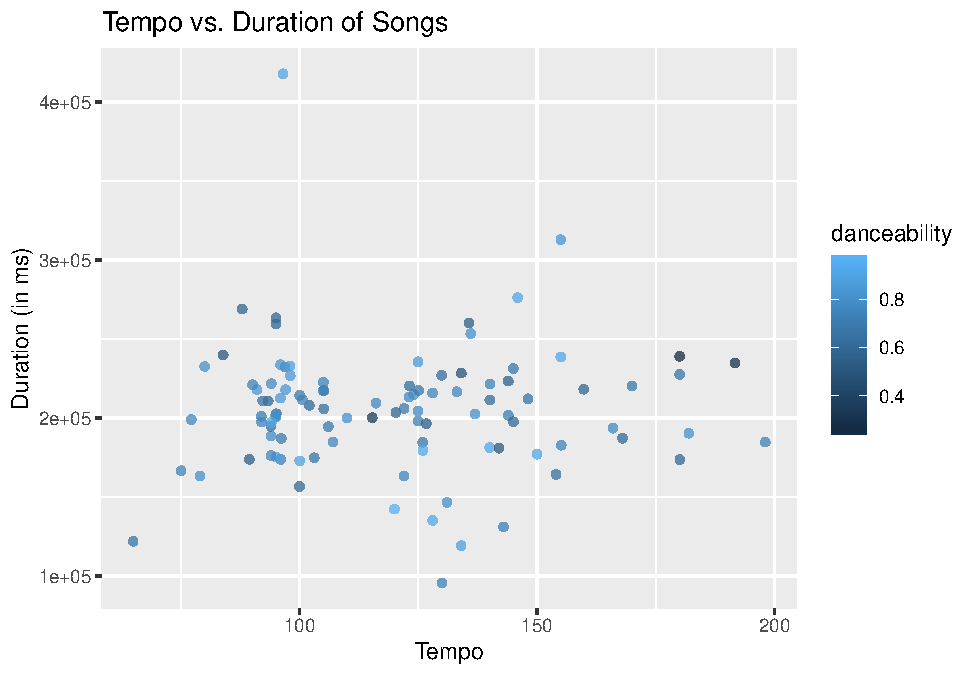
\includegraphics{project2_files/figure-latex/unnamed-chunk-4-1} \end{center}

\begin{Shaded}
\begin{Highlighting}[]
\CommentTok{#linearity and homoskedasticity}
\NormalTok{resids<-}\StringTok{ }\NormalTok{fit}\OperatorTok{$}\NormalTok{residuals}
\NormalTok{fitvals <-}\StringTok{ }\NormalTok{fit}\OperatorTok{$}\NormalTok{fitted.values}
\KeywordTok{ggplot}\NormalTok{()}\OperatorTok{+}\KeywordTok{geom_point}\NormalTok{(}\KeywordTok{aes}\NormalTok{(fitvals, resids))}\OperatorTok{+}\KeywordTok{geom_hline}\NormalTok{(}\DataTypeTok{yintercept =} \DecValTok{0}\NormalTok{, }\DataTypeTok{color =} \StringTok{"red"}\NormalTok{)}
\end{Highlighting}
\end{Shaded}

\begin{center}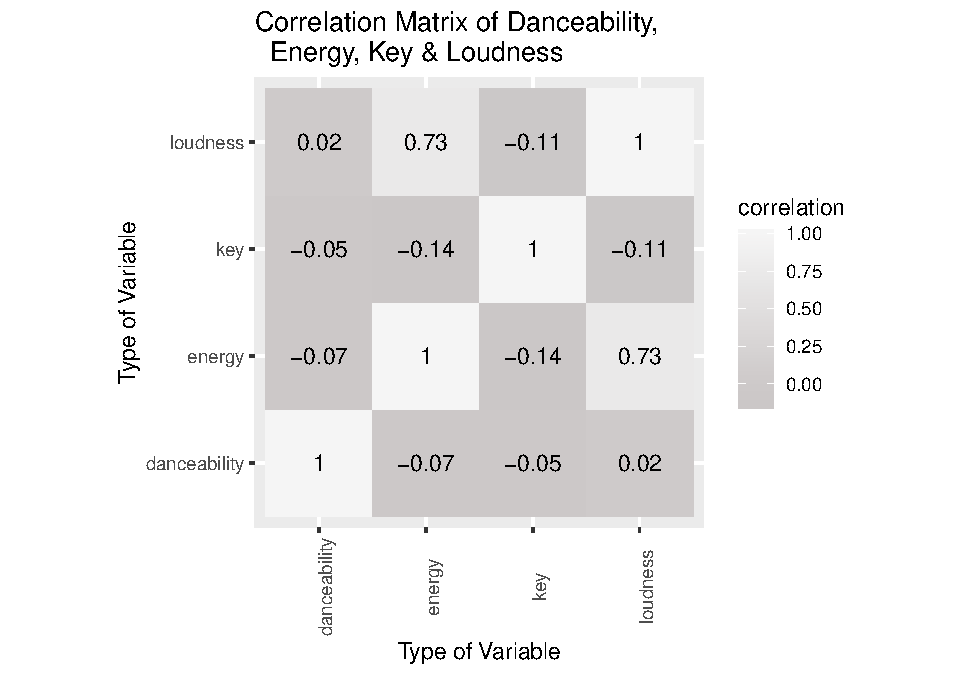
\includegraphics{project2_files/figure-latex/unnamed-chunk-4-2} \end{center}

\begin{Shaded}
\begin{Highlighting}[]
\CommentTok{#normality graphs}
\KeywordTok{ggplot}\NormalTok{()}\OperatorTok{+}\KeywordTok{geom_histogram}\NormalTok{(}\KeywordTok{aes}\NormalTok{(resids),}\DataTypeTok{bins=}\DecValTok{20}\NormalTok{)}
\end{Highlighting}
\end{Shaded}

\begin{center}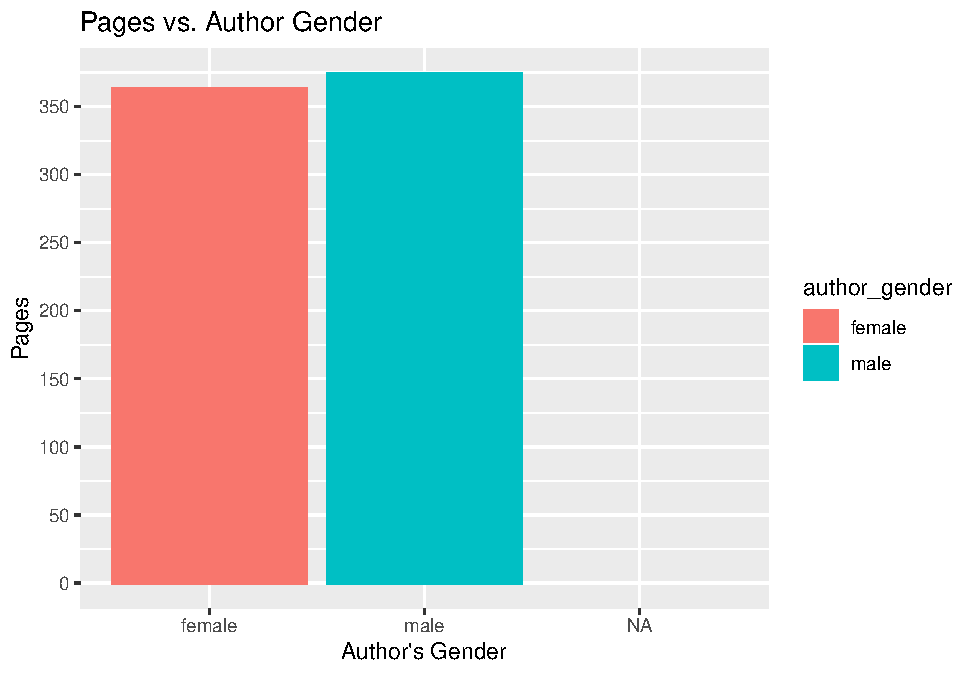
\includegraphics{project2_files/figure-latex/unnamed-chunk-4-3} \end{center}

\begin{Shaded}
\begin{Highlighting}[]
\KeywordTok{ggplot}\NormalTok{()}\OperatorTok{+}\KeywordTok{geom_qq}\NormalTok{(}\KeywordTok{aes}\NormalTok{(}\DataTypeTok{sample=}\NormalTok{resids))}\OperatorTok{+}\KeywordTok{geom_qq_line}\NormalTok{(}\KeywordTok{aes}\NormalTok{(}\DataTypeTok{sample=}\NormalTok{resids), }\DataTypeTok{color=}\StringTok{'red'}\NormalTok{)}
\end{Highlighting}
\end{Shaded}

\begin{center}\includegraphics{project2_files/figure-latex/unnamed-chunk-4-4} \end{center}

\begin{Shaded}
\begin{Highlighting}[]
\KeywordTok{library}\NormalTok{(sandwich);}\KeywordTok{library}\NormalTok{(lmtest)}
\KeywordTok{coeftest}\NormalTok{(fit, }\DataTypeTok{vcov=}\KeywordTok{vcovHC}\NormalTok{(fit))[,}\DecValTok{1}\OperatorTok{:}\DecValTok{4}\NormalTok{]}
\end{Highlighting}
\end{Shaded}

\begin{verbatim}
## Estimate Std. Error t value Pr(>|t|)
## (Intercept) 64.94709075 0.19275962 336.9330695
0.000000e+00
## Gendermale 5.41655493 0.39887856 13.5794586 1.802270e-36
## shoes_c -0.02413067 0.01699139 -1.4201704 1.561196e-01
## Gendermale:shoes_c 0.02253710 0.03730836 0.6040765
5.460397e-01
\end{verbatim}

\hypertarget{bootstrapped-standard-errors}{%
\section{Bootstrapped Standard
Errors}\label{bootstrapped-standard-errors}}

In this section, I reran my same regression model from the previous
section but am going to compute bootstrapped standard errors.
Bootstrapping will allow me to randomly sample rows from my datset with
replcement and calculate coefficient estimates on the bootstrapped
sample.

The bootstrapped SEs are very similar to the robust SEs and the original
SEs for this model. These SEs vary slightly above or slightly below the
robust SEs (above for Gendermale and Gendermale:shoes\_c). However, the
bootstrapped SEs are above the original SEs for the Intercept and the
shoes\_c variables in contrast.

\begin{Shaded}
\begin{Highlighting}[]
\NormalTok{boot_dat<-students[}\KeywordTok{sample}\NormalTok{(}\KeywordTok{nrow}\NormalTok{(students),}\DataTypeTok{replace=}\OtherTok{TRUE}\NormalTok{),]}
\NormalTok{samp_distn<-}\KeywordTok{replicate}\NormalTok{(}\DecValTok{5000}\NormalTok{, \{}
\NormalTok{  boot_dat<-boot_dat<-students[}\KeywordTok{sample}\NormalTok{(}\KeywordTok{nrow}\NormalTok{(students),}\DataTypeTok{replace=}\OtherTok{TRUE}\NormalTok{),]}
\NormalTok{  fit<-}\StringTok{ }\KeywordTok{lm}\NormalTok{(Height}\OperatorTok{~}\NormalTok{Gender}\OperatorTok{*}\NormalTok{shoes_c, }\DataTypeTok{data=}\NormalTok{boot_dat)}
  \KeywordTok{coef}\NormalTok{(fit)}
\NormalTok{\})}
\CommentTok{## Estimated SEs}
\NormalTok{samp_distn}\OperatorTok\NormalTok{t}\OperatorTok\NormalTok{as.data.frame}\OperatorTok\KeywordTok{summarize_all}\NormalTok{(sd)}
\end{Highlighting}
\end{Shaded}

\begin{verbatim}
##   (Intercept) Gendermale    shoes_c Gendermale:shoes_c
## 1   0.1880615  0.4110896 0.01438154         0.03840483
\end{verbatim}

\#Logistic Regression

Next, a logistic regression was performed to try to predict \(y\) from
the variables of Dvds (number of DVDs owned), WakeUp (time they woke
up), and Number (a number that the person randomly chose, from 1-10). I
wanted to see if there was any relationship between these variables and
if the person was male or female.

Based on the logistic regression, the odds of being a male (y = 1), when
Dvds is 0, WakeUp is 0, and Number is 0, is 0.07548153. When controlling
for WakeUp and Number, for every 1 additional increase in number of
Dvds, odds of being a male increase by a factor of 1.00213996. When
controlling for Dvds and Number, for every 1 additional hour increase in
WakeUp time, odds of being a male increase by a factor of 1.23823637.
When controlling for Dvds and WakeUp, for every 1 additional increase in
Number, odds of being a male increase by a factor of 1.01352330.

Next, a confusion matrix was created to compare the model predictions
versus the true outcomes. From this table the accuracy, sensitivity,
specificity and Precision was calculated. In this context, accuracy
would be the proportion of correctly classified cases, sensitivity would
be the proportion of males correctly classified, specificity would be
the proportion of females correctly classified, and precision (or PPV)
would be the proportion of classified males who actually are males. The
accuracy was found to be 0.6601073, sensitivity was 0.06666667,
specificity was 0.978022, and PPV was 0.6190476. Based on these values,
the TNR was very high but the TPR, PPV and accuracy could all be
improved.

Using ggplot, I then plotted the density of log-odds by the \(y\)
variable. Based on this graph, the majority of the gray area is found on
the left of 0, which corresponds with the proportion of false negatives,
where the value is actually male but was predicted to be female. For the
part of the gray area found on the right of 0, this area is the
proportion of females that was predicted as males (false positive).

From the model, I also created an ROC curve/plot to compare TPR to FPR.
Based on this ROC plot and the calculation of AUC, which was found to be
0.591878, we can conclude that this model is a bad predictor overall. In
other words, it is hard to predict Gender from the variables of Dvd,
WakeUp and Number.

Lastly, I performed a 10-fold CV. After first running the class\_diags
function, I set the fold number to 10, created training and test sets,
trained the model on the training set, trained the model on the test set
and then conducted average diagnostics across all k folds. From this
test, the average out-of-sample accuracy, sensitivity and precision
(PPV) was 0.6600325, 0.06505952, and 0.65, respectively. In addition,
the AUC was 0.5900491. Compared to the confusion matrix, these values
are very similar and only differ very slightly.

\begin{Shaded}
\begin{Highlighting}[]
\NormalTok{fit2 <-}\StringTok{ }\KeywordTok{glm}\NormalTok{(y}\OperatorTok{~}\NormalTok{Dvds}\OperatorTok{+}\NormalTok{WakeUp}\OperatorTok{+}\NormalTok{Number, }\DataTypeTok{data =}\NormalTok{ students, }\DataTypeTok{family =} \StringTok{"binomial"}\NormalTok{)}
\KeywordTok{coeftest}\NormalTok{(fit2)}
\end{Highlighting}
\end{Shaded}

\begin{verbatim}
##
## z test of coefficients:
##
## Estimate Std. Error z value Pr(>|z|)
## (Intercept) -2.5838673 0.6074401 -4.2537 2.103e-05 ***
## Dvds 0.0021377 0.0014064 1.5200 0.1285169
## WakeUp 0.2136881 0.0632481 3.3786 0.0007286 ***
## Number 0.0134327 0.0413475 0.3249 0.7452772
## ---
## Signif. codes: 0 '***' 0.001 '**' 0.01 '*' 0.05 '.' 0.1
' ' 1
\end{verbatim}

\begin{Shaded}
\begin{Highlighting}[]
\KeywordTok{exp}\NormalTok{(}\KeywordTok{coef}\NormalTok{(fit2))}
\end{Highlighting}
\end{Shaded}

\begin{verbatim}
## (Intercept)        Dvds      WakeUp      Number 
##  0.07548153  1.00213996  1.23823637  1.01352330
\end{verbatim}

\begin{Shaded}
\begin{Highlighting}[]
\NormalTok{students}\OperatorTok{$}\NormalTok{prob<-}\KeywordTok{predict}\NormalTok{(fit2,}\DataTypeTok{type=}\StringTok{"response"}\NormalTok{)}
\NormalTok{students}\OperatorTok{$}\NormalTok{predicted<-}\KeywordTok{ifelse}\NormalTok{(students}\OperatorTok{$}\NormalTok{prob}\OperatorTok{>}\NormalTok{.}\DecValTok{5}\NormalTok{,}\StringTok{"male"}\NormalTok{,}\StringTok{"female"}\NormalTok{)}
\NormalTok{students}\OperatorTok{$}\NormalTok{Gender<-}\KeywordTok{factor}\NormalTok{(students}\OperatorTok{$}\NormalTok{Gender,}\DataTypeTok{levels=}\KeywordTok{c}\NormalTok{(}\StringTok{"female"}\NormalTok{,}\StringTok{"male"}\NormalTok{))}

\KeywordTok{table}\NormalTok{(}\DataTypeTok{truth=}\NormalTok{students}\OperatorTok{$}\NormalTok{Gender, }\DataTypeTok{prediction=}\NormalTok{students}\OperatorTok{$}\NormalTok{predicted)}\OperatorTok\NormalTok{addmargins}
\end{Highlighting}
\end{Shaded}

\begin{verbatim}
##         prediction
## truth    female male Sum
##   female    356    8 364
##   male      182   13 195
##   Sum       538   21 559
\end{verbatim}

\begin{Shaded}
\begin{Highlighting}[]
\CommentTok{#accuracy}
\NormalTok{(}\DecValTok{356}\OperatorTok{+}\DecValTok{13}\NormalTok{)}\OperatorTok{/}\DecValTok{559}
\end{Highlighting}
\end{Shaded}

\begin{verbatim}
## [1] 0.6601073
\end{verbatim}

\begin{Shaded}
\begin{Highlighting}[]
\CommentTok{#sensitivity (TPR)}
\DecValTok{13}\OperatorTok{/}\DecValTok{195}
\end{Highlighting}
\end{Shaded}

\begin{verbatim}
## [1] 0.06666667
\end{verbatim}

\begin{Shaded}
\begin{Highlighting}[]
\CommentTok{#specificity (TNR)}
\DecValTok{356}\OperatorTok{/}\DecValTok{364}
\end{Highlighting}
\end{Shaded}

\begin{verbatim}
## [1] 0.978022
\end{verbatim}

\begin{Shaded}
\begin{Highlighting}[]
\CommentTok{#precision (PPV)}
\DecValTok{13}\OperatorTok{/}\DecValTok{21}
\end{Highlighting}
\end{Shaded}

\begin{verbatim}
## [1] 0.6190476
\end{verbatim}

\begin{Shaded}
\begin{Highlighting}[]
\NormalTok{students}\OperatorTok{$}\NormalTok{logit<-}\KeywordTok{predict}\NormalTok{(fit2) }\CommentTok{#get predicted log-odds}
\KeywordTok{ggplot}\NormalTok{(students,}\KeywordTok{aes}\NormalTok{(logit, }\DataTypeTok{fill=}\NormalTok{Gender))}\OperatorTok{+}\KeywordTok{geom_density}\NormalTok{(}\DataTypeTok{alpha=}\NormalTok{.}\DecValTok{3}\NormalTok{)}\OperatorTok{+}
\StringTok{  }\KeywordTok{geom_vline}\NormalTok{(}\DataTypeTok{xintercept=}\DecValTok{0}\NormalTok{,}\DataTypeTok{lty=}\DecValTok{2}\NormalTok{)}
\end{Highlighting}
\end{Shaded}

\begin{center}\includegraphics{project2_files/figure-latex/unnamed-chunk-6-1} \end{center}

\begin{Shaded}
\begin{Highlighting}[]
\KeywordTok{library}\NormalTok{(plotROC)}
\NormalTok{ROCplot <-}\StringTok{ }\KeywordTok{ggplot}\NormalTok{(students)}\OperatorTok{+}\KeywordTok{geom_roc}\NormalTok{(}\KeywordTok{aes}\NormalTok{(}\DataTypeTok{d =}\NormalTok{ y, }\DataTypeTok{m =}\NormalTok{ prob), }\DataTypeTok{n.cuts =} \DecValTok{0}\NormalTok{)}
\NormalTok{ROCplot}
\end{Highlighting}
\end{Shaded}

\begin{center}\includegraphics{project2_files/figure-latex/unnamed-chunk-6-2} \end{center}

\begin{Shaded}
\begin{Highlighting}[]
\KeywordTok{calc_auc}\NormalTok{(ROCplot)}
\end{Highlighting}
\end{Shaded}

\begin{verbatim}
##   PANEL group      AUC
## 1     1    -1 0.591878
\end{verbatim}

\begin{Shaded}
\begin{Highlighting}[]
\CommentTok{#K-fold CV}
\NormalTok{class_diag<-}\ControlFlowTok{function}\NormalTok{(probs,truth)\{}
  
\NormalTok{  tab<-}\KeywordTok{table}\NormalTok{(}\KeywordTok{factor}\NormalTok{(probs}\OperatorTok{>}\NormalTok{.}\DecValTok{5}\NormalTok{,}\DataTypeTok{levels=}\KeywordTok{c}\NormalTok{(}\StringTok{"FALSE"}\NormalTok{,}\StringTok{"TRUE"}\NormalTok{)),truth)}
\NormalTok{  acc=}\KeywordTok{sum}\NormalTok{(}\KeywordTok{diag}\NormalTok{(tab))}\OperatorTok{/}\KeywordTok{sum}\NormalTok{(tab)}
\NormalTok{  sens=tab[}\DecValTok{2}\NormalTok{,}\DecValTok{2}\NormalTok{]}\OperatorTok{/}\KeywordTok{colSums}\NormalTok{(tab)[}\DecValTok{2}\NormalTok{]}
\NormalTok{  spec=tab[}\DecValTok{1}\NormalTok{,}\DecValTok{1}\NormalTok{]}\OperatorTok{/}\KeywordTok{colSums}\NormalTok{(tab)[}\DecValTok{1}\NormalTok{]}
\NormalTok{  ppv=tab[}\DecValTok{2}\NormalTok{,}\DecValTok{2}\NormalTok{]}\OperatorTok{/}\KeywordTok{rowSums}\NormalTok{(tab)[}\DecValTok{2}\NormalTok{]}

  \ControlFlowTok{if}\NormalTok{(}\KeywordTok{is.numeric}\NormalTok{(truth)}\OperatorTok{==}\OtherTok{FALSE} \OperatorTok{&}\StringTok{ }\KeywordTok{is.logical}\NormalTok{(truth)}\OperatorTok{==}\OtherTok{FALSE}\NormalTok{) truth<-}\KeywordTok{as.numeric}\NormalTok{(truth)}\OperatorTok{-}\DecValTok{1}
  
  \CommentTok{#CALCULATE EXACT AUC}
\NormalTok{  ord<-}\KeywordTok{order}\NormalTok{(probs, }\DataTypeTok{decreasing=}\OtherTok{TRUE}\NormalTok{)}
\NormalTok{  probs <-}\StringTok{ }\NormalTok{probs[ord]}
\NormalTok{  truth <-}\StringTok{ }\NormalTok{truth[ord]}
 
\NormalTok{  TPR=}\KeywordTok{cumsum}\NormalTok{(truth)}\OperatorTok{/}\KeywordTok{max}\NormalTok{(}\DecValTok{1}\NormalTok{,}\KeywordTok{sum}\NormalTok{(truth)) }
\NormalTok{  FPR=}\KeywordTok{cumsum}\NormalTok{(}\OperatorTok{!}\NormalTok{truth)}\OperatorTok{/}\KeywordTok{max}\NormalTok{(}\DecValTok{1}\NormalTok{,}\KeywordTok{sum}\NormalTok{(}\OperatorTok{!}\NormalTok{truth))}
  
\NormalTok{  dup<-}\KeywordTok{c}\NormalTok{(probs[}\OperatorTok{-}\DecValTok{1}\NormalTok{]}\OperatorTok{>=}\NormalTok{probs[}\OperatorTok{-}\KeywordTok{length}\NormalTok{(probs)], }\OtherTok{FALSE}\NormalTok{)}
\NormalTok{  TPR<-}\KeywordTok{c}\NormalTok{(}\DecValTok{0}\NormalTok{,TPR[}\OperatorTok{!}\NormalTok{dup],}\DecValTok{1}\NormalTok{)}
\NormalTok{  FPR<-}\KeywordTok{c}\NormalTok{(}\DecValTok{0}\NormalTok{,FPR[}\OperatorTok{!}\NormalTok{dup],}\DecValTok{1}\NormalTok{)}
  
\NormalTok{  n <-}\StringTok{ }\KeywordTok{length}\NormalTok{(TPR)}
\NormalTok{  auc<-}\StringTok{ }\KeywordTok{sum}\NormalTok{( ((TPR[}\OperatorTok{-}\DecValTok{1}\NormalTok{]}\OperatorTok{+}\NormalTok{TPR[}\OperatorTok{-}\NormalTok{n])}\OperatorTok{/}\DecValTok{2}\NormalTok{) }\OperatorTok{*}\StringTok{ }\NormalTok{(FPR[}\OperatorTok{-}\DecValTok{1}\NormalTok{]}\OperatorTok{-}\NormalTok{FPR[}\OperatorTok{-}\NormalTok{n]) )}

  \KeywordTok{data.frame}\NormalTok{(acc,sens,spec,ppv,auc)}
\NormalTok{\}}

\KeywordTok{set.seed}\NormalTok{(}\DecValTok{1234}\NormalTok{)}
\NormalTok{k=}\DecValTok{10}

\NormalTok{data<-students[}\KeywordTok{sample}\NormalTok{(}\KeywordTok{nrow}\NormalTok{(students)),] }
\NormalTok{folds<-}\KeywordTok{cut}\NormalTok{(}\KeywordTok{seq}\NormalTok{(}\DecValTok{1}\OperatorTok{:}\KeywordTok{nrow}\NormalTok{(students)),}\DataTypeTok{breaks=}\NormalTok{k,}\DataTypeTok{labels=}\NormalTok{F) }

\NormalTok{diags<-}\OtherTok{NULL}
\ControlFlowTok{for}\NormalTok{(i }\ControlFlowTok{in} \DecValTok{1}\OperatorTok{:}\NormalTok{k)\{}
  \CommentTok{## Create training and test sets}
\NormalTok{  train<-data[folds}\OperatorTok{!=}\NormalTok{i,] }
\NormalTok{  test<-data[folds}\OperatorTok{==}\NormalTok{i,]}
\NormalTok{  truth<-test}\OperatorTok{$}\NormalTok{y}
  
  \CommentTok{## Train model on training set}
\NormalTok{  fit2 <-}\StringTok{ }\KeywordTok{glm}\NormalTok{(y}\OperatorTok{~}\NormalTok{Dvds}\OperatorTok{+}\NormalTok{WakeUp}\OperatorTok{+}\NormalTok{Number, }\DataTypeTok{data =}\NormalTok{ students, }\DataTypeTok{family =} \StringTok{"binomial"}\NormalTok{) }
\NormalTok{  probs<-}\KeywordTok{predict}\NormalTok{(fit2,}\DataTypeTok{newdata =}\NormalTok{ test,}\DataTypeTok{type=}\StringTok{"response"}\NormalTok{)}
  
  \CommentTok{## Test model on test set (save all k results)}
\NormalTok{  diags<-}\KeywordTok{rbind}\NormalTok{(diags,}\KeywordTok{class_diag}\NormalTok{(probs,truth))}
\NormalTok{\}}
\KeywordTok{summarize_all}\NormalTok{(diags,mean)}
\end{Highlighting}
\end{Shaded}

\begin{verbatim}
##         acc       sens      spec       ppv       auc
## 1 0.6600649 0.06861175 0.9778893 0.6166667 0.5941437
\end{verbatim}

\hypertarget{lasso-regression}{%
\section{LASSO Regression}\label{lasso-regression}}

For this last regression, I chose the variable of \(y\) to predict from
the rest of my variables. After running this lasso regression, I found
out that the variables of Height, Shoes, ToSleep, WakeUp and Haircut are
all important predictors of \(y\).

Next, I performed a 10-fold CV using this new model with only the
important predictors. From this cross validation test, I got an accuracy
value of 0.9158442, a sensitivity value of 0.8905952, a specificity
value of 0.9349463, a PPV value of 0.8770614, and an AUC value of
0.9568835. Compared to the logistic regression completed in the previous
section, this 10-fold CV was much more accurate, specific and an overall
better predictor of the \(y\) variable. This is probably due to using
the variables that are most important in predicting \(y\), which was
found through the lasso function.

\begin{Shaded}
\begin{Highlighting}[]
\NormalTok{students}\OperatorTok{$}\NormalTok{Gender <-}\StringTok{ }\OtherTok{NULL}
\NormalTok{students}\OperatorTok{$}\NormalTok{shoes_c <-}\StringTok{ }\OtherTok{NULL}
\NormalTok{students}\OperatorTok{$}\NormalTok{prob <-}\StringTok{ }\OtherTok{NULL}
\NormalTok{students}\OperatorTok{$}\NormalTok{predicted<-}\StringTok{ }\OtherTok{NULL}
\NormalTok{students}\OperatorTok{$}\NormalTok{logit<-}\StringTok{ }\OtherTok{NULL}

\NormalTok{fit3<-}\KeywordTok{glm}\NormalTok{(y}\OperatorTok{~}\NormalTok{., }\DataTypeTok{data =}\NormalTok{ students, }\DataTypeTok{family =} \StringTok{"binomial"}\NormalTok{)}

\KeywordTok{set.seed}\NormalTok{(}\DecValTok{1234}\NormalTok{)}
\NormalTok{x<-}\KeywordTok{model.matrix}\NormalTok{(fit3)}
\NormalTok{y<-}\KeywordTok{as.matrix}\NormalTok{(students}\OperatorTok{$}\NormalTok{y)}

\KeywordTok{library}\NormalTok{(glmnet)}
\NormalTok{cv<-}\KeywordTok{cv.glmnet}\NormalTok{(x,y, }\DataTypeTok{family =} \StringTok{"binomial"}\NormalTok{)}
\NormalTok{lasso<-}\KeywordTok{glmnet}\NormalTok{(x,y,}\DataTypeTok{lambda=}\NormalTok{cv}\OperatorTok{$}\NormalTok{lambda}\FloatTok{.1}\NormalTok{se)}
\KeywordTok{coef}\NormalTok{(lasso)}
\end{Highlighting}
\end{Shaded}

\begin{verbatim}
## 12 x 1 sparse Matrix of class "dgCMatrix"
##                       s0
## (Intercept) -2.931764867
## (Intercept)  .          
## Height       0.050506949
## Shoes       -0.007753662
## Number       .          
## Dvds         .          
## ToSleep      0.009777990
## WakeUp       0.010973130
## Haircut     -0.002541920
## Job          .          
## Drinkpop     .          
## Drinkwater  -0.011656570
\end{verbatim}

\begin{Shaded}
\begin{Highlighting}[]
\CommentTok{#10-fold CV}
\KeywordTok{set.seed}\NormalTok{(}\DecValTok{1234}\NormalTok{)}
\NormalTok{data1 <-}\StringTok{ }\NormalTok{students }\OperatorTok\StringTok{ }\NormalTok{sample_frac}
\NormalTok{folds1 <-}\StringTok{ }\KeywordTok{ntile}\NormalTok{(}\DecValTok{1}\OperatorTok{:}\KeywordTok{nrow}\NormalTok{(students),}\DataTypeTok{n=}\DecValTok{10}\NormalTok{)}

\NormalTok{diags1<-}\OtherTok{NULL}
\ControlFlowTok{for}\NormalTok{(i }\ControlFlowTok{in} \DecValTok{1}\OperatorTok{:}\NormalTok{k)\{}
\NormalTok{  train1<-}\StringTok{ }\NormalTok{data1[folds}\OperatorTok{!=}\NormalTok{i,] }\CommentTok{#create training set (all but fold i)}
\NormalTok{  test1<-}\StringTok{ }\NormalTok{data1[folds}\OperatorTok{==}\NormalTok{i,] }\CommentTok{#create test set (just fold i)}
\NormalTok{  truth1<-}\StringTok{ }\NormalTok{test1}\OperatorTok{$}\NormalTok{y }\CommentTok{#save truth labels from fold i}
  
\NormalTok{  fit4 <-}\StringTok{ }\KeywordTok{glm}\NormalTok{(y}\OperatorTok{~}\NormalTok{Height}\OperatorTok{+}\NormalTok{Shoes}\OperatorTok{+}\NormalTok{ToSleep}\OperatorTok{+}\NormalTok{WakeUp}\OperatorTok{+}\NormalTok{Haircut, }\DataTypeTok{data=}\NormalTok{train1, }\DataTypeTok{family=}\StringTok{"binomial"}\NormalTok{)}
\NormalTok{  probs1 <-}\StringTok{ }\KeywordTok{predict}\NormalTok{(fit4, }\DataTypeTok{newdata=}\NormalTok{test1, }\DataTypeTok{type=}\StringTok{"response"}\NormalTok{)}
  
\NormalTok{  diags1<-}\KeywordTok{rbind}\NormalTok{(diags1,}\KeywordTok{class_diag}\NormalTok{(probs1,truth1))}
\NormalTok{\}}

\KeywordTok{summarize_all}\NormalTok{(diags1,mean)}
\end{Highlighting}
\end{Shaded}

\begin{verbatim}
##         acc      sens      spec       ppv       auc
## 1 0.9159416 0.8812861 0.9311269 0.8854968 0.9533547
\end{verbatim}

\emph{This concludes the end of my project 2.}

\end{document}
